\section{Introduction}
\label{sec:introduction}
\paragraph{}
\par The goal of this laboratory assignment is to study and analyse a RC circuit composed by a dependent current source, a capacitor, resistors, and  lastly, one dependent and one independent voltage source to find the natural and forced response and frequency analysis of the said circuit.
A comparison will be done between the NgSpice simulation and the theoretical analysis of the circuit.
\par The main objective will be to further learn about both methods of analysis, learning about their similarities, differences and which positive and negative sides each of them have. 
\par The circuit is represented with resort to \textit{LibreOffice Draw} and can be viewed in figure \ref{circuit}.

\begin{figure}[H]
    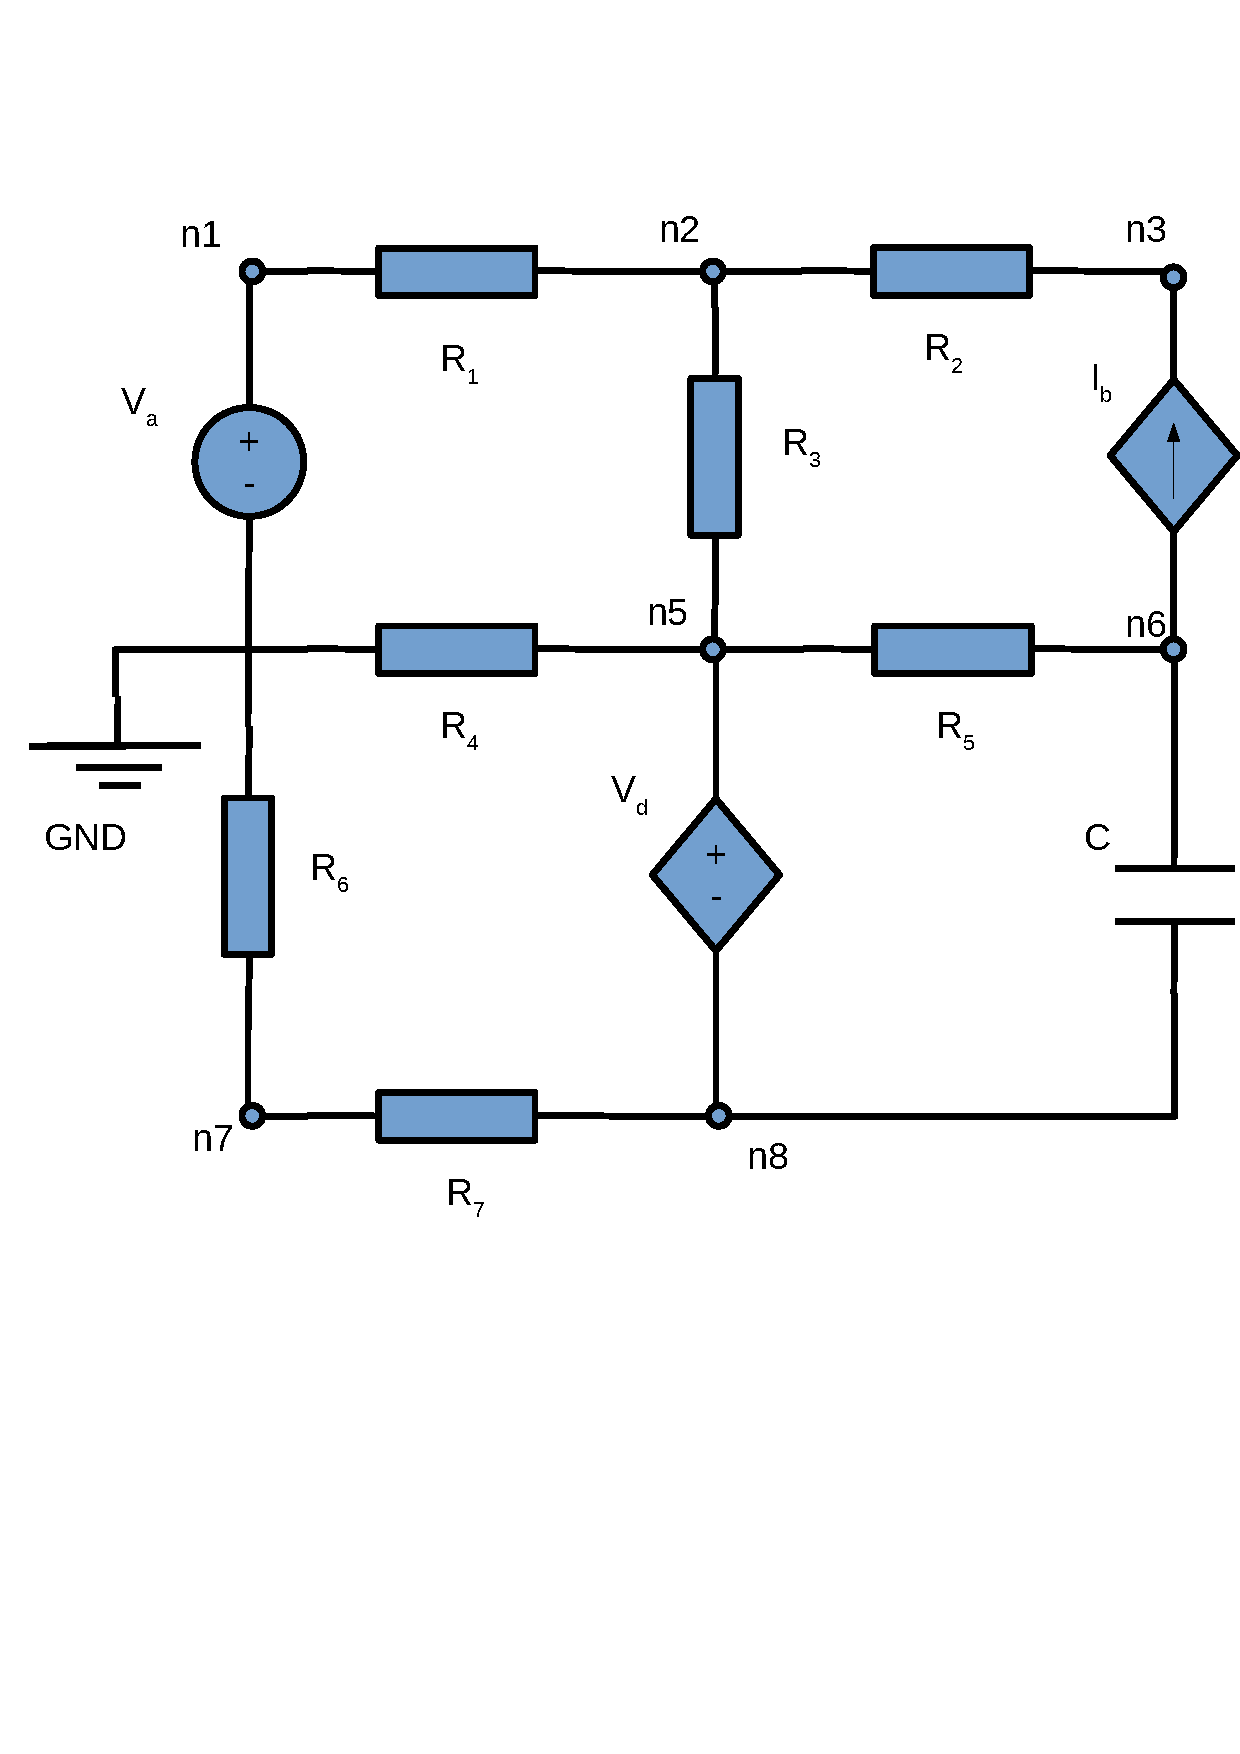
\includegraphics[width=0.5\linewidth]{Lab2.pdf}
    \centering
    \caption{Studied Circuit}
    \label{circuit}
\end{figure}


In Section~\ref{sec:analysis}, a theoretical analysis of the circuit is
presented. In Section~\ref{sec:simulation}, the circuit is analysed by
simulation, and the results are compared to the theoretical results obtained in
Section~\ref{sec:analysis}. The conclusions of this study are outlined in
Section~\ref{sec:conclusion}.
